%!TEX root=paper.tex

\newpage
\section{How Do Students Use the Possibility of Reading Personally Interesting Articles?}
\label{sec:results}

% \subsection {Feed Subscriptions}
Figure \ref{fig:registrations} represents an incidence matrix collected at the end of the study interval: the columns represent students, and the rows represent news feeds; if a student is registered to a given feed, at the intersection of the corresponding row and column we place $\Diamond$. 

We would expect to see fully continuous horizontal rows of data-points if every user subscribed to the same feed, and fully continuous vertical rows if every user subscribed to all of the feeds available. The notion that these patterns are largely absent in Figure 4 supports our assumption that different individuals prefer to subscribe to different reading sources.

The figure illustrates that giving the students the freedom to choose the sources they wanted, allowed each one of them to express their interest. 

\begin{figure}[h!]
\centering
  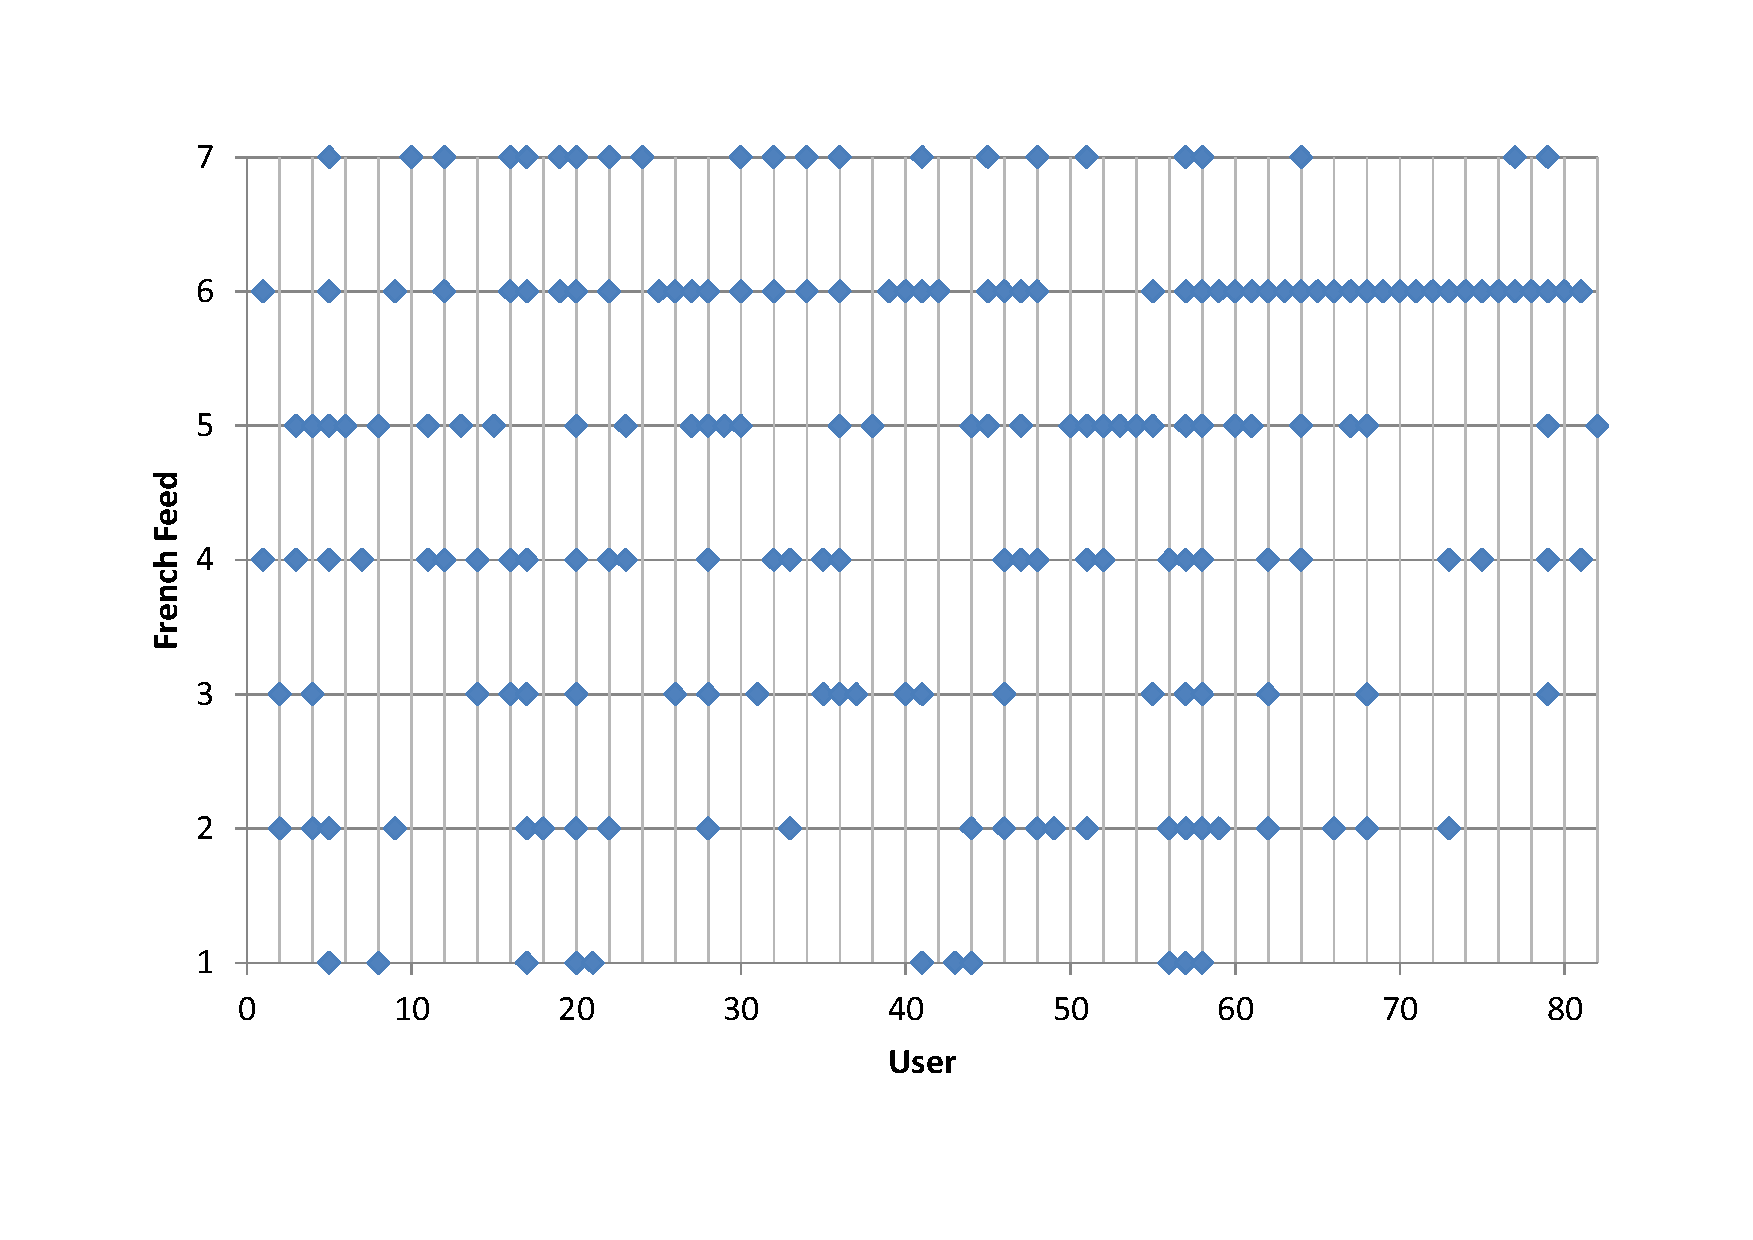
\includegraphics[width=\columnwidth]{figures/users_feeds}
  \caption{Different users subscribe to different sources}~\label{fig:registrations}
\end{figure}

Of course some feeds are more popular than others. Projecting the data- points into the vertical axis and sorting the results leaves us with a histogram as can be seen in Figure 5.

\begin{figure}[h!]
\centering
  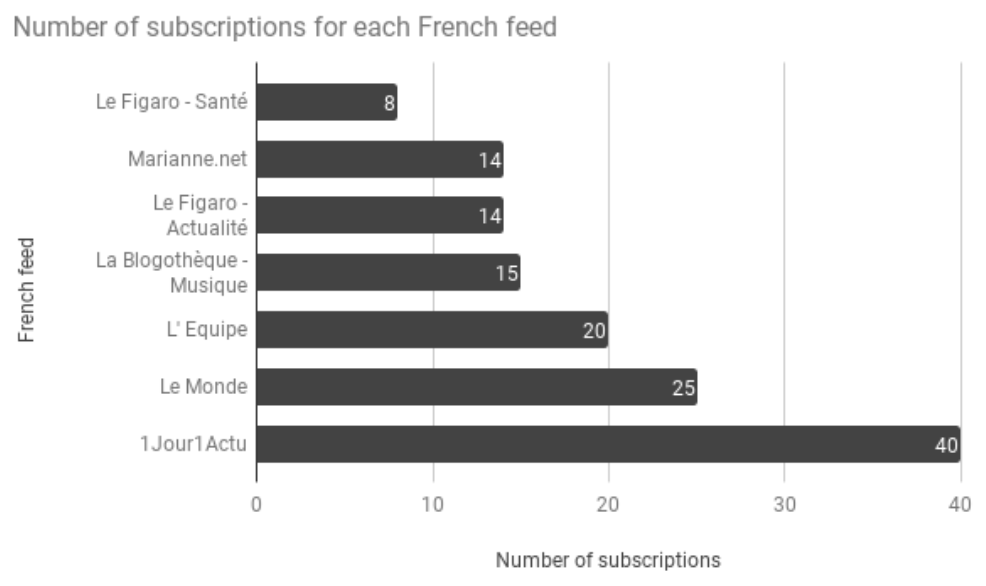
\includegraphics[width=\columnwidth]{figures/feed_popularity}
  \caption{Some feeds are more popular than others}~\label{fig:registrations}
\end{figure}


Feed {\em 1Jour1Actu} is the most popular French feed, and feed Le Figaro - Sant\'e is the least popular French feed. In order to see whether or not this might be related to how they are presented in the dialog window of our system (see Figure \ref{fig:system_subscriptions}), we can compare the order of popularity with the order in which they are displayed.

\begin{figure}[h!]
\centering
  \newcommand{\picscale}{0.5}
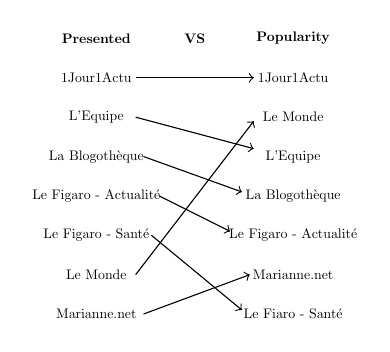
\begin{tikzpicture}[scale=\picscale, every node/.style={scale=\picscale}]
    % Columns.
    \node at (0  , 0) {\bf Presented};
    \node at (2.5, 0) {\bf VS};
    \node at (5  , 0) {\bf Popularity};
    
    % As presented.
    \node at (0,-1) {1Jour1Actu};
    \node at (0,-2) {L'Equipe};
    \node at (0,-3) {La Blogoth\`{e}que};
    \node at (0,-4) {Le Figaro - Actualit\'{e}};
    \node at (0,-5) {Le Figaro - Sant\'{e}};
    \node at (0,-6) {Le Monde};
    \node at (0,-7) {Marianne.net};
    
    % As popular.
    \node at (5,-1) {1Jour1Actu};
    \node at (5,-2) {Le Monde};
    \node at (5,-3) {L'Equipe};
    \node at (5,-4) {La Blogoth\`{e}que};
    \node at (5,-5) {Le Figaro - Actualit\'{e}};
    \node at (5,-6) {Marianne.net};
    \node at (5,-7) {Le Fiaro - Sant\'{e}};
    
    % Arrows between presented and popular.
    \draw [->] (1,-1)   --   (4,-1);
    \draw [->] (1,-2)   --   (4,-2.8);
    \draw [->] (1.2,-3) --   (3.7,-3.9);
    \draw [->] (1.6,-4) --   (3.4,-4.9);
    \draw [->] (1.4,-5) --   (3.7,-6.9);
    \draw [->] (1,-6)   --   (4,-2.1);
    \draw [->] (1.2,-7) --   (3.9,-6);
    
\end{tikzpicture} 
  \caption{The popularity of the feeds vs. their ranking in the UI}~\label{fig:registrations}
\end{figure}

One can see how the second-to-last presented feed, Le Monde, is the second most popular feed by measure of subscriptions. Conversely, the feed listed above Le Monde is actually the least subscribed-to feed in our listing.

\subsection{Article Interactions}
If we investigate the articles that the users interact with, we see the same pattern: each user explores their own interest, and there is no one article that is interesting for all of them. \ml{Can we provide a bit more information: which article is read by the most people, and how many people is that? Maybe we could sort this not by article ID, but reorder the article lines, in such a way that the most popular ones are at the bottom and the most unique ones at the top?}

\begin{figure}[h!]
\centering
  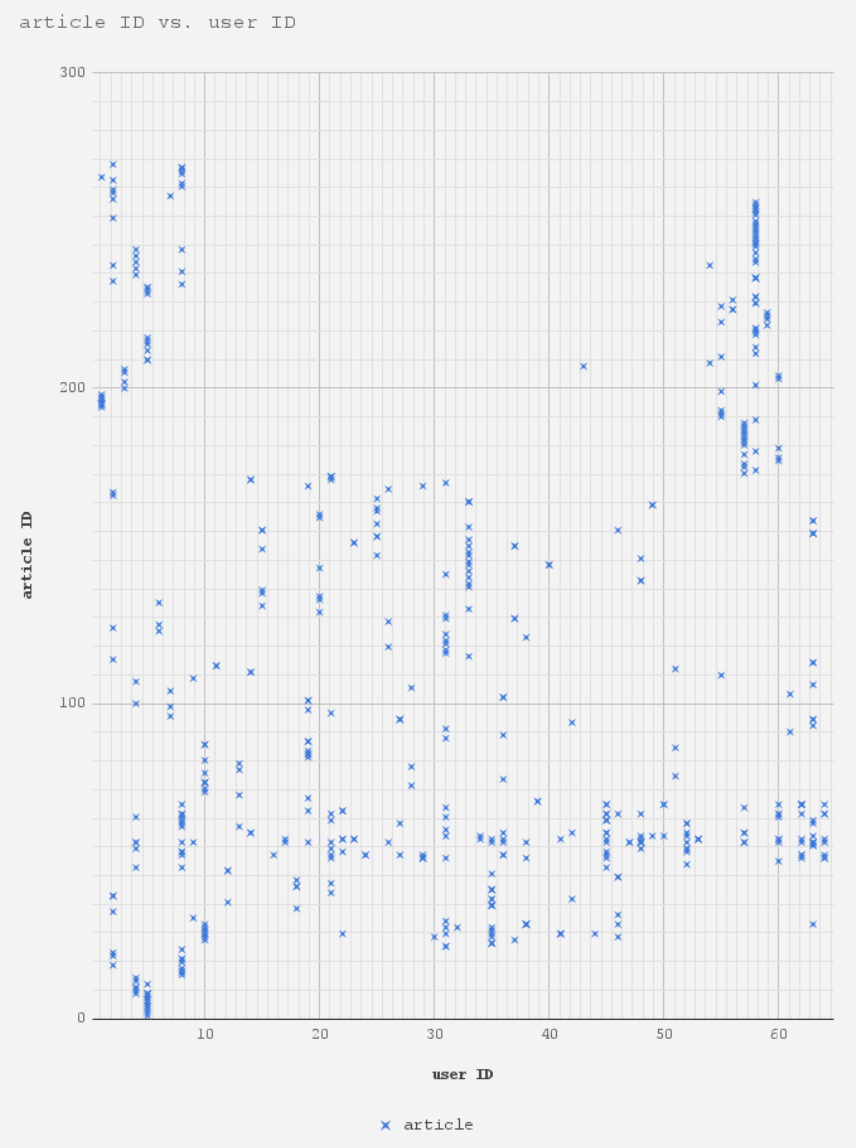
\includegraphics[width=0.8\columnwidth]{figures/users_articles}
  \caption{Every student has their own article reading preferences}~\label{fig:registrations}
\end{figure}

\subsection{Which Interactive Features Are Most Used?}
We tracked the usage of the various features in the interactive reader through a telemetry system that records all the interactions with a set of interactive elements of interest. Figure \ref{fig:feature_usage} shows the most used features of the system. With 6700 occurrences, requesting a translation for a word is the most used interactive feature of the system. The second most used feature is opening the ``translation alternatives'' menu. The ratio of translations to alternate translation requests is six to one. 

The third most used feature is the text to speech feature. On average, there are about 1.66 pronunciations for a given selection, suggesting that users are often asking for a second pronunciation after hearing it the first time. \ml{@dan, do you agree with this conclusion?}

Undo-ing a translation is used when the user wants to remove the translation that he just added to the text. This seems to be a very popular action too. 

A Like button (\rightthumbsup) can be found at the bottom of an article and it was clicked by the readers 174 times. This information is not used anywhere for now, although we plan to use it in the future for improving text recommendations and adding information about the number of ``likes'' other readers rated an article with. 


\begin{figure}[h!]
\centering
  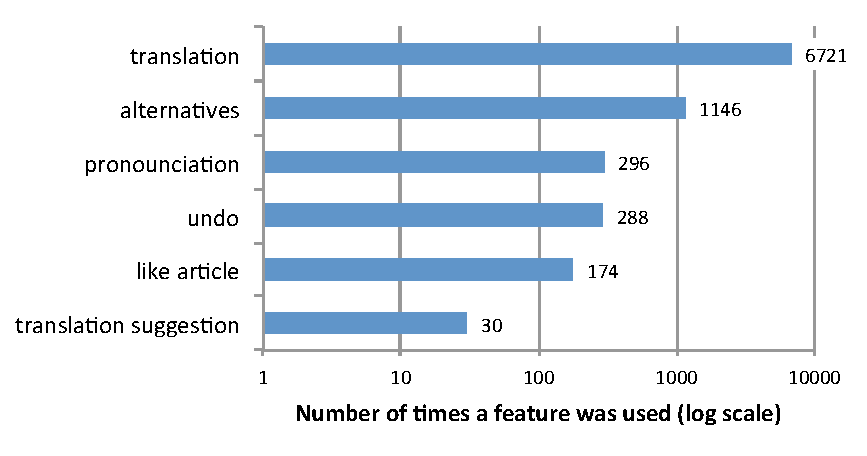
\includegraphics[width=0.8\columnwidth]{figures/reader_feature_usage}
  \caption{Popularity of features by their recorded usage-events}
  \label{fig:feature_usage}
\end{figure}

\ml{like -- what does it mean for design? can we verify that they actually read those articles. how many did they read and didn't like?}

To see how widespread the various features are among our users, we also looked at the number of distinct users for each category of events. A larger number of distinct users indicates that the feauture is useful to the broadest number of students.

\begin{figure}[h!]
\centering
  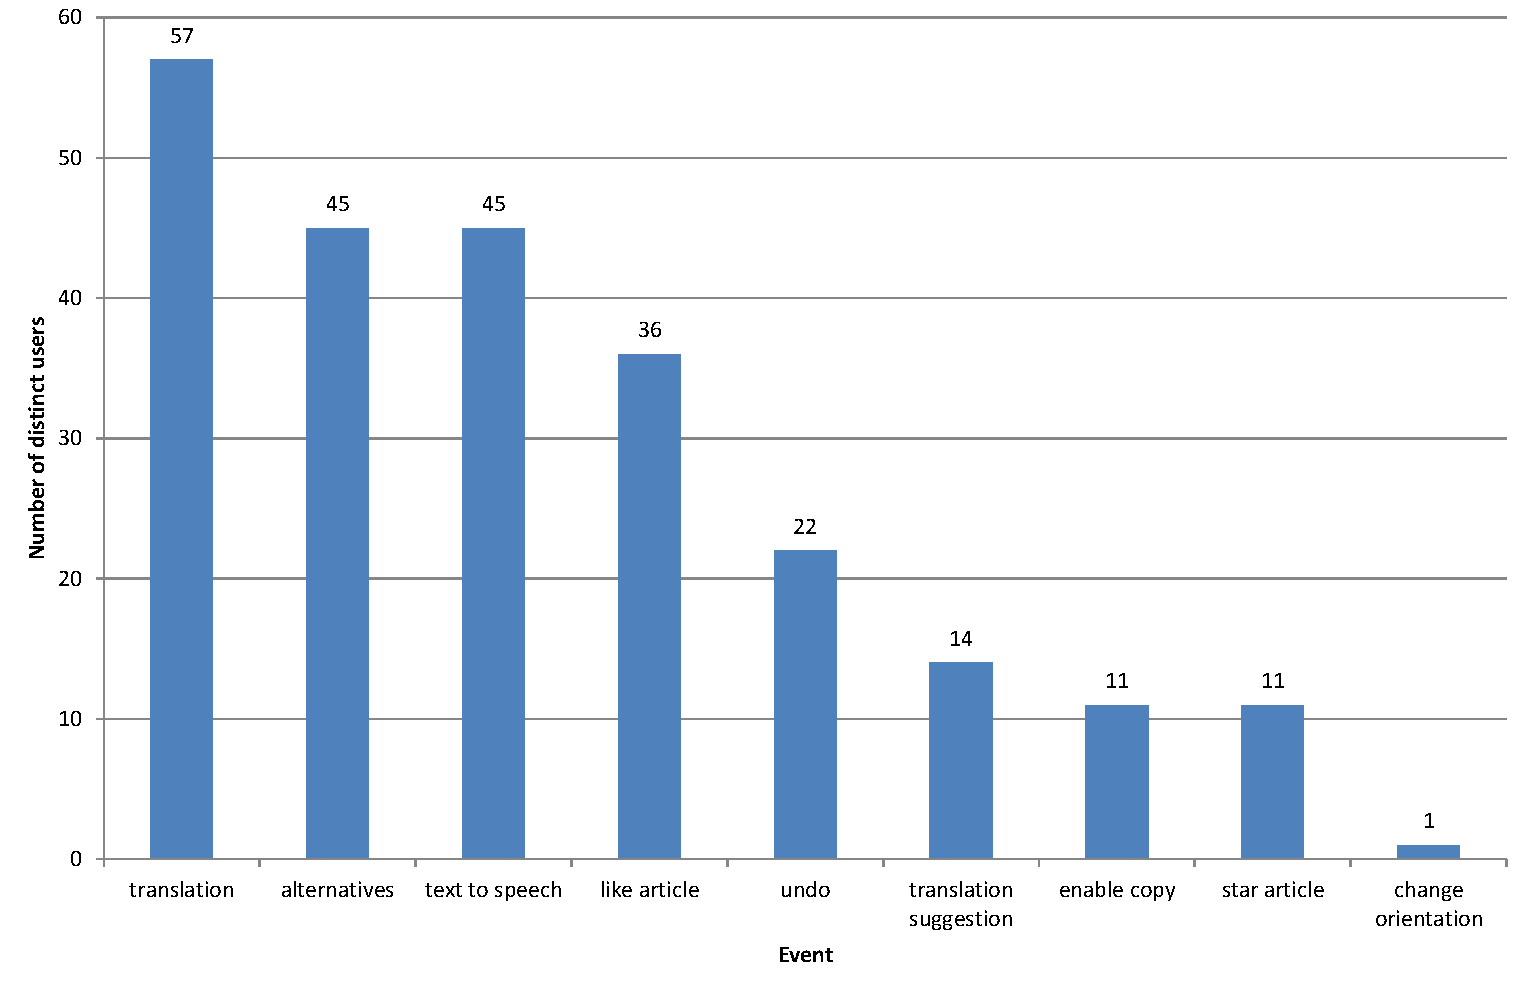
\includegraphics[width=0.8\columnwidth]{figures/reader_feature_usage_per_user}
  \caption{The usage of the various reader features by the various users }
\end{figure}

In addition, we looked at the number of times the same word or phrase was pronounced by the same user. This data ranges from one single pronunciation to 14 pronunciations for the same word (phrase). The size of this interval is mostly due to the users' different proficiency in a certain language and the difficulty in pronunciation of the word (phrase) itself. Nevertheless, on average, the number approaches 1.66 pronunciation requests for the same
piece of text, suggesting that users are generally sufficiently content with a pronunciation after hearing it the first time.



\section{How Do Students Use the Personalized Vocabulary Exercises?}

The personalized exercises are a complement to the reading. 

The system presented four types of vocabulary practice exercises to the students. In total, during the entire duration of the study we observed 18.082 exercises being presented to the students, leading to an average of 300 exercises per student. Figure \ref{fig:ex_interactions} shows one outlier student who did 3.000 (!) exercises during one month, and about six over-eager students who did close to 700 exercises. 

The figure also highlights the difference between exercises which had a ``correct'' outcome vs. exercises which had a ``wrong'' outcome. 


  \begin{figure}[h!]
  \centering
    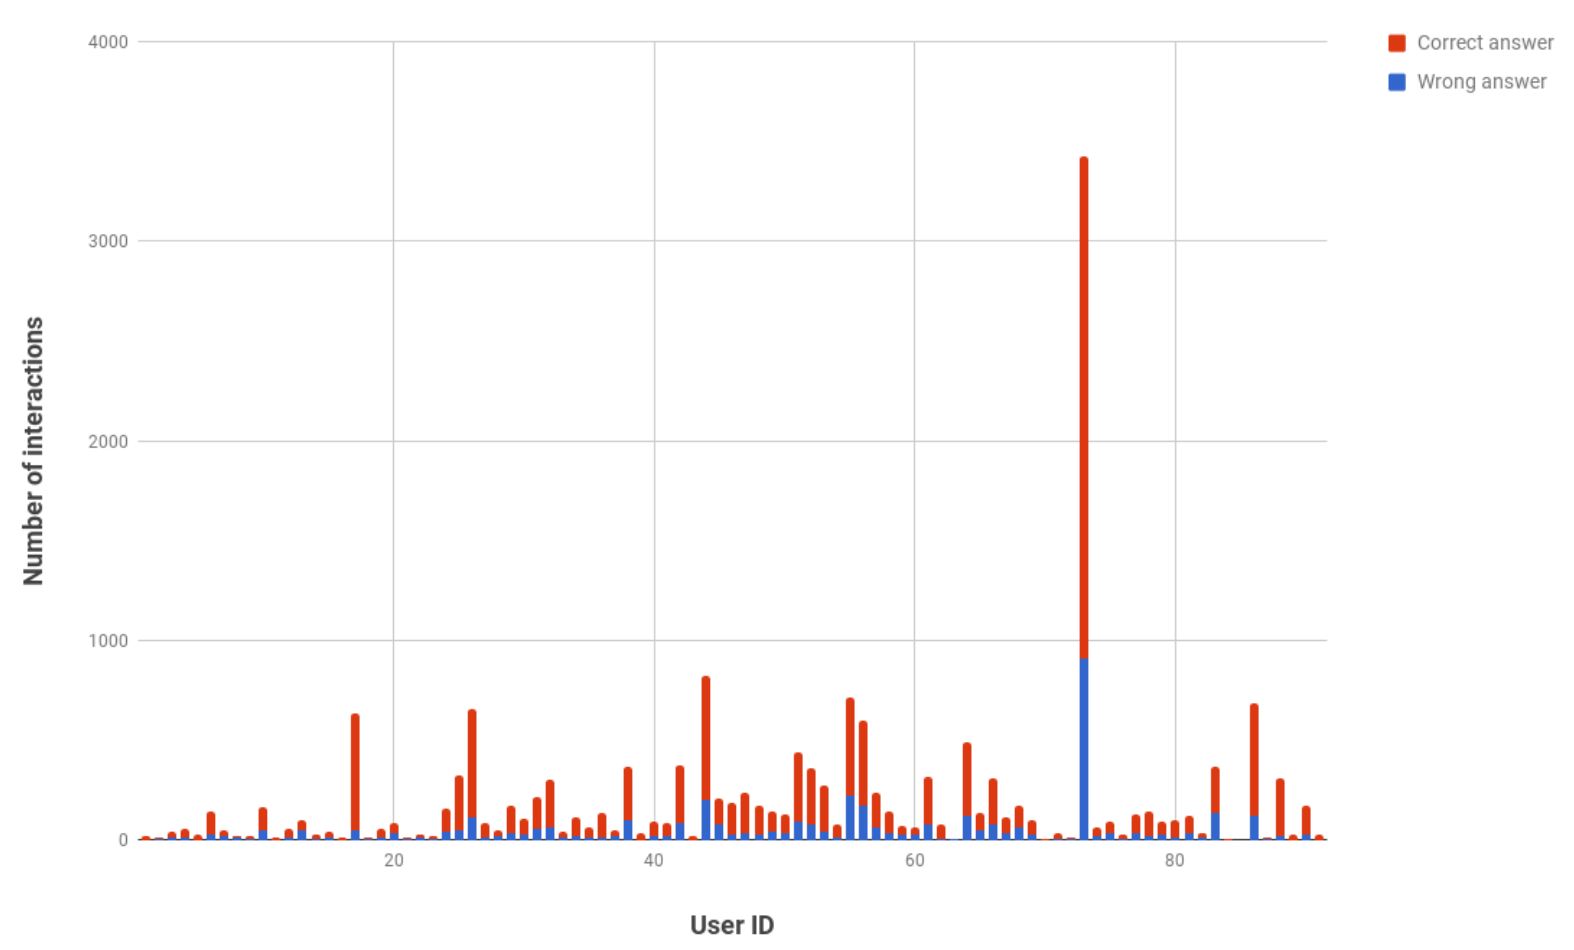
\includegraphics[width=\columnwidth]{figures/exercise_interactions_count.png}
    \caption{Some students are much more motivated than others in doing exercises }
    \label{fig:ex_interactions}
  \end{figure}


% \begin{tabular}{lrrrr}
%   % source id: 
%   % choose -- 5
%   % find -- 4
%   % translate -- 7
%   % match -- 6
%                       & Choose  & Find & Translate & Match \\ \hline
%   Total interactions  & 7180    & 6249 & 2643      & 2010\\
%   Hint requests       & 29      & 529  & 847       & 16 \\ \hline
% \end{tabular}

Figure \ref{fig:activity_per_day} shows in which days are the individual learners using the exercises. What we see is a distribution over the entire period of the study, with a slightly more intensive period towards the end of the period which might signify cramming before the end of the semester.

  \begin{figure}[h!]
  \centering
    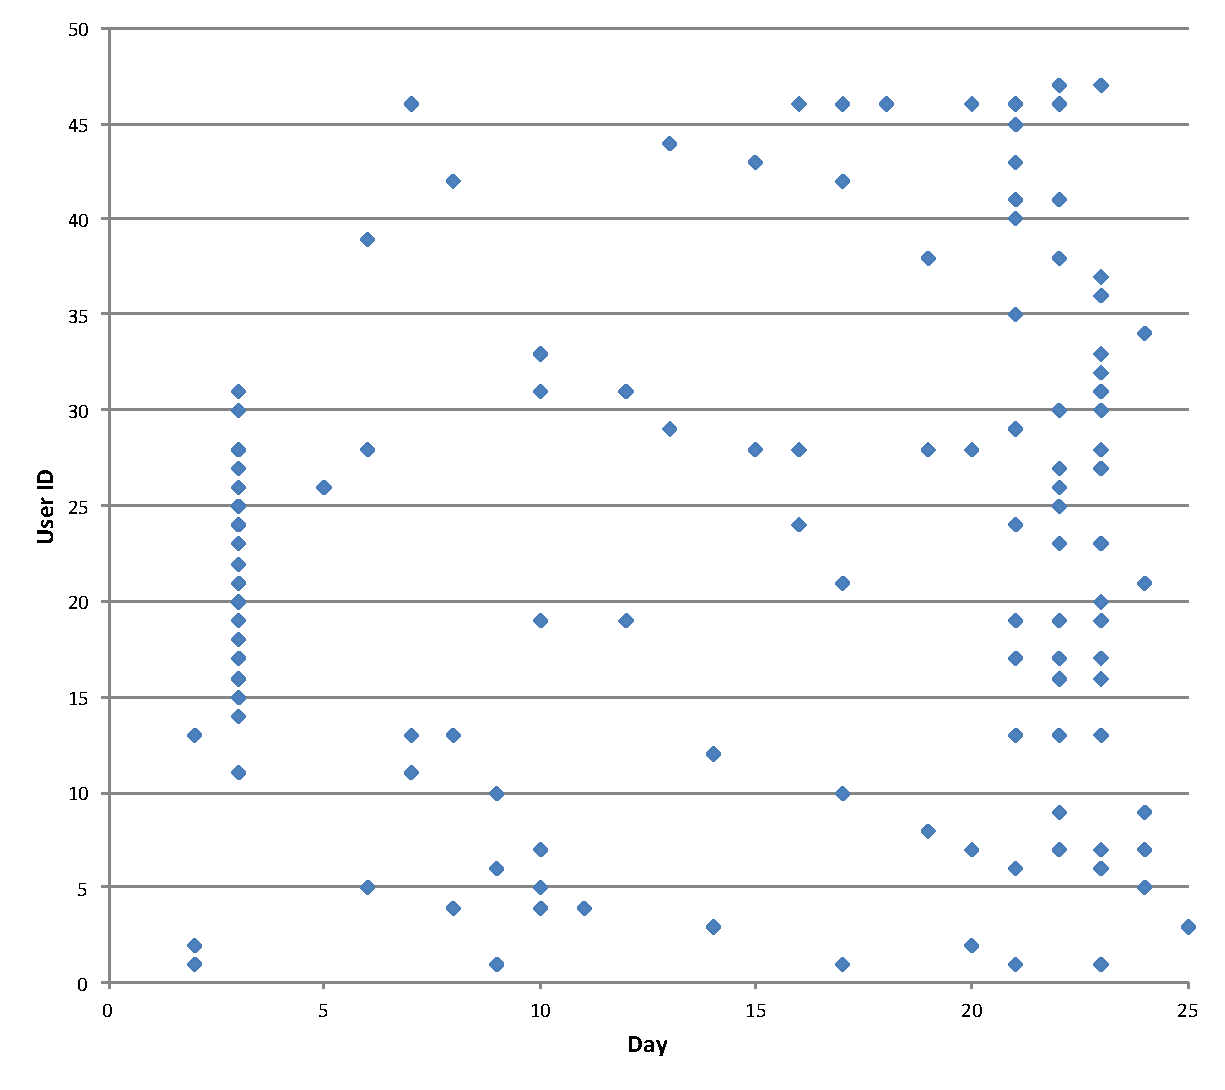
\includegraphics[width=\columnwidth]{figures/user_exercise_activity_vs_day.pdf}
    \caption{The students are doing exercises at their own pace throughout the one month interval }
    \label{fig:activity_per_day}
  \end{figure}

\newpage
\section{What is the Perception of the Learners?}

\subsection{In App Feedback Request}
Besides the analysis that we did based on the observed user data, we also asked the students a series of questions by popping up questions while they are using the sytem (by using an online tool called HotJar). Among the questions was whether they preferred the reading platform and why. Some of the qnswers can be seen in the screenshot below. It becomes clear that the students appreciate the possibility of reading what is interesting for them.

    \begin{figure}[h!]
    \centering
      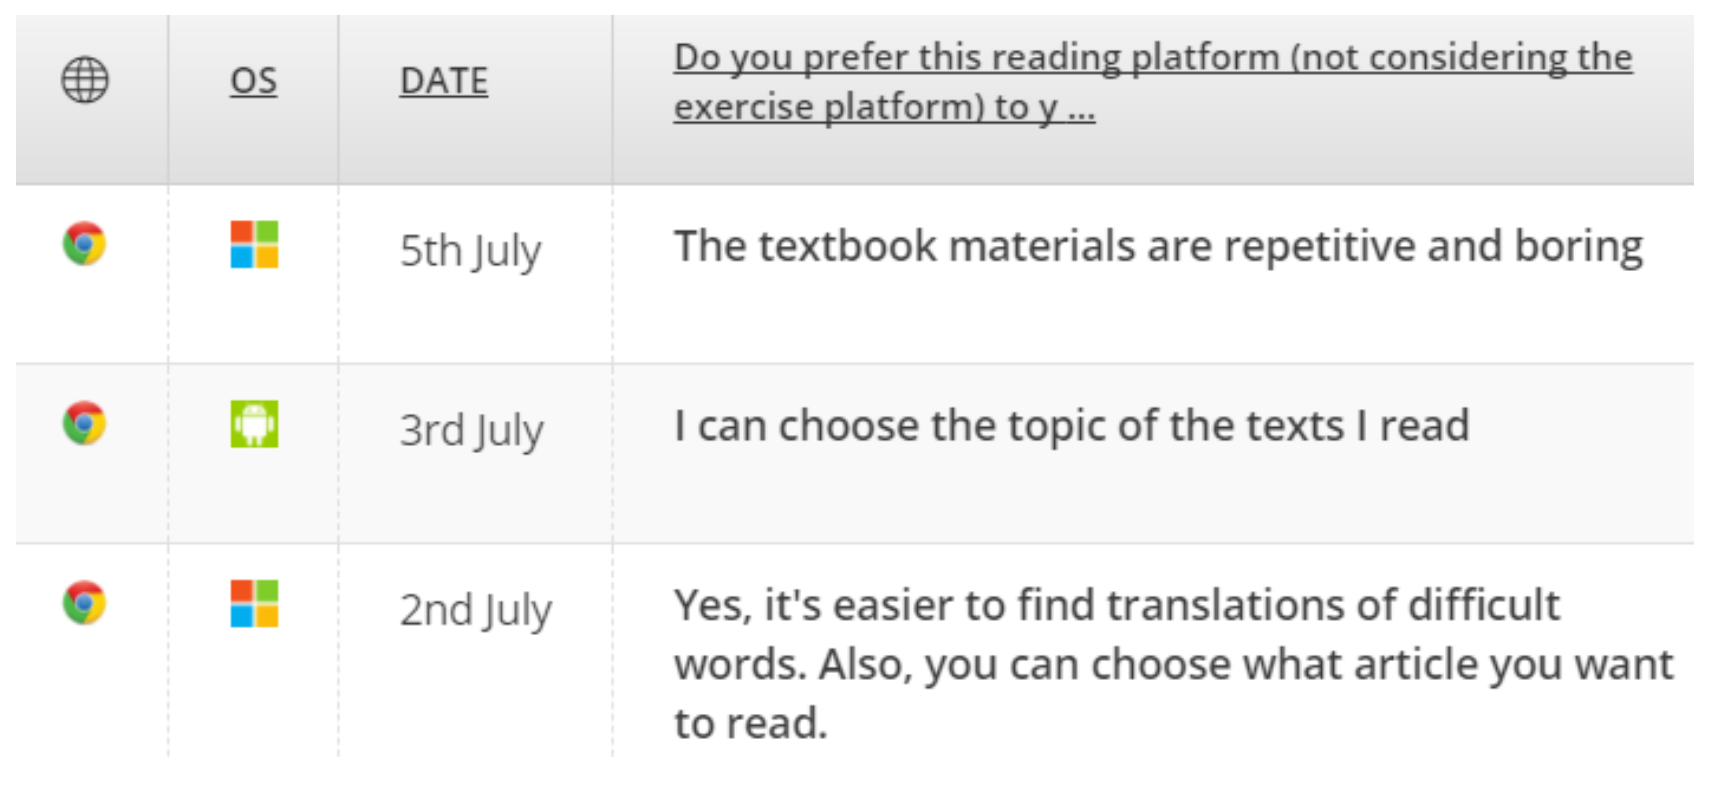
\includegraphics[width=0.9\columnwidth]{figures/opinion_on_reading_platform}
      \caption{The students appreciate the freedom of reading what is interesting to them }
    \end{figure}

\subsection{Post-Usage Survey}

The majority of the students who answered our post-usage survey said that  they prefer our system to a textbook. However, we still think this is not very conclusive since the number of students who answered our survey was quite limited: 12 of the 60 students represent about 20\% of the participants. 


\subsection{Reports to the Teacher}
However, since they might have been more sincere when reporting to their teacher than directly to us, we report here also what they wrote in a separate evaluation of the tools they use in the class, which the teacher runs always at the end of the school year. Several of the answers are: 

\begin{description}
  \item {\em ``It works well but it were better if the translation would have been in Dutch. It is good that you can choose yourself what to read.''}
  \item {\em ``Good for reading skills. It would have been best if it were in Dutch.''}
  \item {\em ``Your vocabulary is really moving forward, but then you have to do it more often than a few times. Overall a nice website, easy and fun subjects''}
\end{description}

There main message in the feedback is that learners appreciate the freedom of chosing materials to read that are personally interesting for them. The second, implied observation is that they appreciate the translations, but they would want to have them in their native language. 

% The way forward is then, by providing better recommendations if possible, and by providing translations in their native languages.

% In the future we plan to investigate whether the system works well enough with Dutch.

\newpage
\section{Limitations of this Study}
\label{sec:limitations}
% We presented a system, and we showed that it has the potential to generate user involvement. However the study we performed is not sufficient to reach a strong conclusion about the impact of the system we present... 

The feedback from the users was positive. However, they might have been influenced by our enthusiastic presentation of the system at the begining of the testing month. 



We showed that the users are using the system extensively. However, this might be because the students had to use the system as part of their assignment in the class. We showed that the majority of the students used the system constantly throughout the one month period. If they only used it for a grade, we would have expected a more focused cramming at the end of the period (which we actually saw with a few of the students, but not with the majority). 

The students we worked with are not necesarily representative for the Dutch highschool student population since they are bilingual. Even in this case, during the fedback multiple of them opined that they would prefer to use the system in their native Dutch as opposed to English.

% We observed that students prefer to interact with different texts...  

The algorithms for scheduling vocabulary exercises are the state of the art in spaced repetition. However, we did not have a control group to see whether this approach works better than others. Moreover, note that other approaches for using spaced repetition already exist; what is unique in our approach is that the students learn based on personalized exercises generated based on the context of their past readings.






